\documentclass{article}
\usepackage{graphicx}

\begin{document}
\title{TBA Assignment}
\author{Joris Slob}
\date{October 2014}
\maketitle

\section{Introduction}

The following subsections have been copied from the original problem
statement that was sent to me.

\subsection{Problem Statement}

\subsubsection{Introduction}

In this assignment you are asked to model the process of trucks
arriving at a container terminal gate, moving to a handling location
where they can either receive or deliver a container from a stack
crane, and driving back to the exit gate to exit the terminal. The
modelling of this system should be done in Java, and the result to be
delivered is the Java application and source code as well as a short
report describing the approach and answering the main research
question.

\subsubsection{Problem Formulation}

Trucks arrive at the terminal in the pattern described in the attached
file TruckActivity.xlsx. A DLVR or RECV move is indicated from the
point of view of the terminal: DLVR means the truck comes to the
terminal to pick up a container, and RECV indicates the terminal
receives a container, so the truck brings one in.

The entry gate consists of several lanes where an arriving truck can
be processed. Each gate lane has a separate queue associated with
it. At each lane, the processing time of a truck in minutes is
described by the random variable $X_1$, where $X_1 \sim Gamma(9, 3)$,
where 9 is the shape parameter $\alpha$ and 3 is the rate parameter
$\beta$, and $E(X_1) = \alpha / \beta$.

The truck then proceeds to one of 10 stack modules. Driving from the
gate to the stacks or vice-versa takes 3 minutes. The stack modules
can be represented as a system of 10 servers, having one single
queue. Each server is able to handle one truck at a time. Any truck
can be served by any of the servers. The service time $X_2 \sim
Gamma(4, 2)$.

After service at the stack module, the truck drives to the exit
gate. Handling time at the exit gate $X_3 \sim Gamma(3, 3)$. As with
the entry gate, each gate lane has a separate queue associated with
it.

The terminal operator has indicated that the maximum queue length at
any point during the day should not exceed 30 trucks.

\subsubsection{Assignment}

How many lanes at the entry and exit gate would you advise the
terminal to use?

\subsection{Additional questions asked}

Before starting with the assignment I asked some additional questions.

\begin{itemize}
\item Can I use github to host my code?
\item Can I assume that the truck arrival pattern will remain the same
  in the future?
\item Can I assume none of the trucks have priority?
\item Is the date in the TruckActivity.xlsx file in the format
  year/month/day?
\item In which timezone is the harbor located?
\end{itemize}

The answers I received back were:

\begin{itemize}
\item I can use github if I do not actively advertise that the
  assignment and code is there.
\item I can assume the arrival pattern will remain the same in the
  future.
\item None of the trucks have higher priority.
\item The format is indeed year/month/day
\item Timezone is not relevant, but assume Netherlands.
\end{itemize}

\subsection{Approach}

In the methods section I describe in more detail how I approached this
problem. To determine the approach I would take I first did some
simple calculations to see what I could expect. For this I took the
xlsx file and quick estimate of the solution.

First observation is that the entries in the xlsx file are all for one
day. The first truck arrives at the harbor at $T_1$ 06:02:29 and the
last truck arrives at $T_{1327}$ 15:24:16. That means that 1327 trucks
arrive in 561.78 minutes for an average of 2.36 trucks/min.

To deal with this load every part of the harbor has to be able to deal
with this load. The entry gate takes 3 minutes on average to deal with
a truck, so to handle 2.36 trucks/min requires $2.36 / 1/3 = 7.08$
lanes. The stack modules take 2 minutes on average to deal with trucks
and there are ten, so they can handle 5 trucks/min. We expect no
problems for this estimate there. The exit gate takes 1 minute on
average to deal with a truck, so to handle the 2.36 trucks/min
requires 2.36 lanes.

Let us model this gate problem in software to verify these results.

\section{Method}

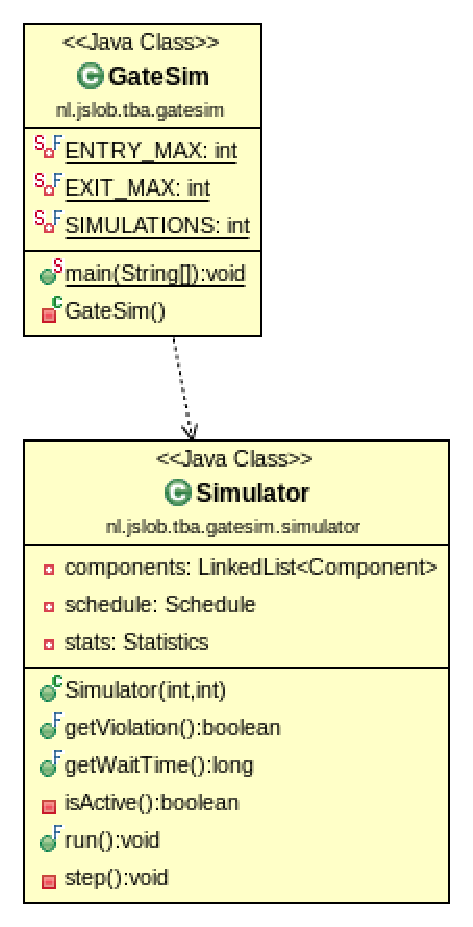
\includegraphics[scale=0.5]{GateSim.eps}
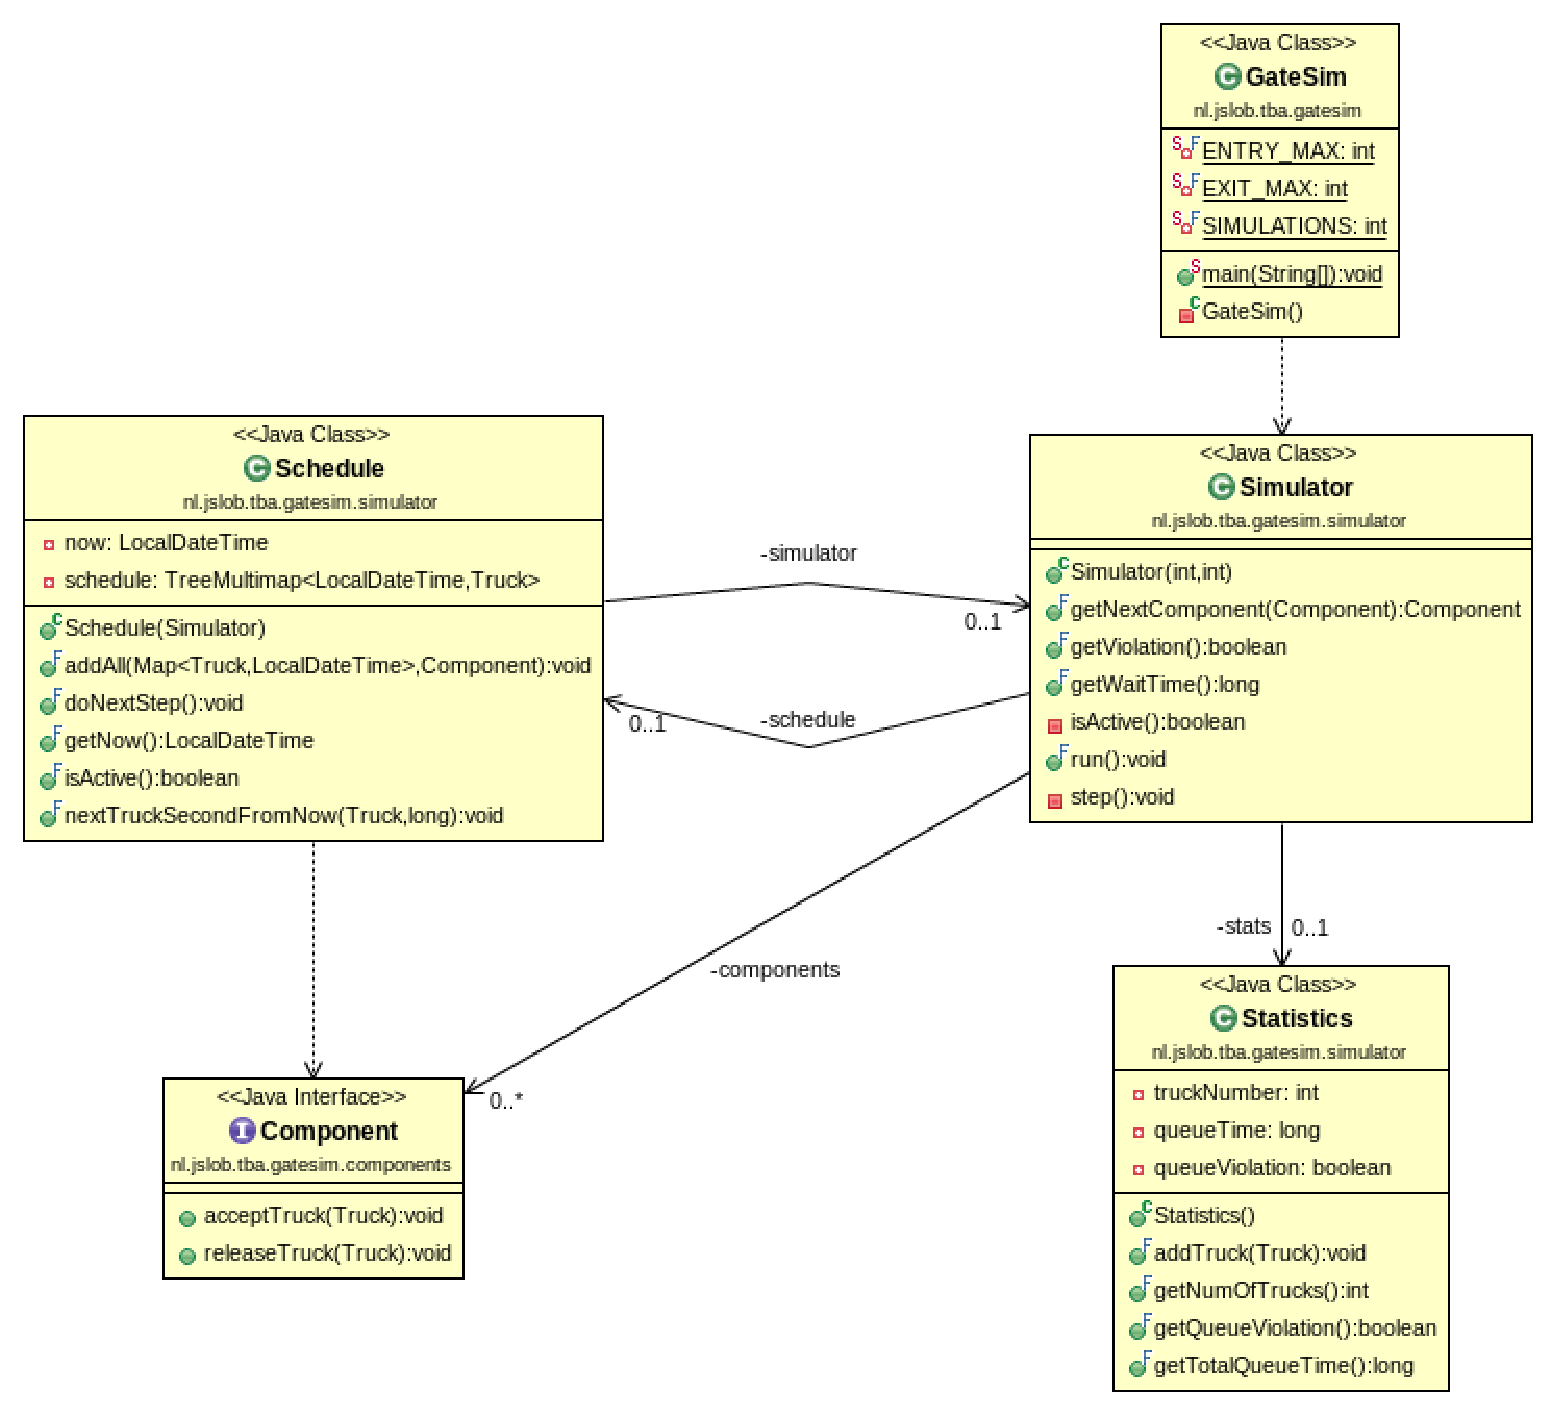
\includegraphics[scale=0.5]{Simulator.eps}

\section{Results}


\section{Discussion}

The first result that satisfies the assignment is the model with 7
entry lanes and 3 exit lanes. This comes close to the initial estimate
given in the introduction. In this assignment we have introduced
another metric to evaluate the performance of the system:
TotalQueueWaitingTime. With data on the total time lost in queues the
harbor can consider opening more lanes to compensate truck waiting
time. Opening new lanes and operating them also has a cost, but these
were not given in the assignment.

This simulation is embarrassingly parallel and could be made to run
several simulations in separate threads.

\end{document}
